\documentclass{article}
\usepackage{iclr2026_conference,times}
\input{math_commands.tex}
\usepackage{hyperref}
\usepackage{url}
\usepackage{booktabs}
\usepackage{graphicx}
\title{Energy Guidance Does Not Create Missing Diffusion-Policy Support}
\author{Anonymous Authors}
\begin{document}
\maketitle

\begin{abstract}
We rebuilt a generated robotics idea into a falsifiable trajectory-diffusion study: does energy guidance during reverse diffusion create new safe robot behavior, or does it merely re-rank samples already supported by the policy prior? The v4 rebuild implements a planar continuous-control benchmark with obstacle and dynamics constraints, offline demonstration support gaps, a kernel reverse-diffusion trajectory sampler, energy re-ranking, guided diffusion, safety-projected guidance, CEM trajectory optimization, a grid oracle, seven seeds, ablations, stress sweeps, and negative cases. The result is negative. On the decisive \texttt{off\_support\_corridor} split, where the safe homotopy is absent from the diffusion prior and the demonstrated homotopy is blocked, \texttt{energy\_guided\_diffusion} reaches $0.000 \pm 0.000$ success, exactly matching \texttt{energy\_rerank\_unguided}. CEM and the oracle both reach $1.000 \pm 0.000$. The paired guided-minus-rerank success difference is $0.000$, and guided-minus-CEM is $-1.000$. We therefore mark the paper \textbf{KILL/ARCHIVE} for ICLR main.
\end{abstract}

\section{Decision}
This document is the v4 ICLR-main gate for Paper 78, \emph{Energy-Guided Diffusion Policy Limits}. The previous version was killed because it only contained synthetic template evidence. The current rebuild adds an implemented local benchmark and stronger baselines. The rejection reason has changed: evidence now exists, but it refutes the central submission claim.

\section{Hypothesis}
The tested hypothesis is that energy guidance during reverse diffusion can change reachable behavior beyond sample re-ranking. In robotics terms, a guided diffusion policy should be able to move from an unsafe or blocked demonstrated homotopy to a different safe homotopy when the task energy reveals that the demonstrated mode is no longer feasible. The paper passes the local gate only if guided diffusion improves over energy re-ranking and is competitive with a strong trajectory optimizer while preserving collision and dynamics safety.

\section{Benchmark}
The benchmark is a 2D end-effector trajectory task with start and goal states, circular obstacles, velocity limits, smoothness limits, and offline demonstrations. Demonstrations define the support of the diffusion prior. The runner evaluates five splits: \texttt{supported\_single\_mode}, \texttt{supported\_multimodal\_shift}, \texttt{rare\_mode\_recovery}, \texttt{off\_support\_corridor}, and \texttt{deceptive\_energy\_basin}. The decisive split is \texttt{off\_support\_corridor}: demonstrations use a lower corridor, the lower corridor is blocked at test time, and the safe upper corridor is geometrically feasible but absent from the prior.

The full run contains 980 main rollout rows, 245 seed-level metric rows, 392 ablation rollout rows, and 420 stress-sweep rollout rows. Intervals are 95 percent confidence intervals over seed-level means.

\section{Methods}
The implemented methods are:
\begin{itemize}
\item \texttt{behavior\_clone\_nearest}: nearest demonstration trajectory.
\item \texttt{unguided\_diffusion\_prior}: kernel denoising reverse-diffusion sampler over demonstrations.
\item \texttt{energy\_rerank\_unguided}: draws unguided diffusion samples and chooses the lowest task energy.
\item \texttt{energy\_guided\_diffusion}: applies task-energy gradients during every denoising step.
\item \texttt{strong\_guided\_diffusion}: adds more conservative guidance and safety projection.
\item \texttt{cem\_trajectory\_optimizer}: cross-entropy trajectory optimizer using the same task constraints.
\item \texttt{grid\_oracle}: coarse geometric upper bound.
\end{itemize}

\section{Main Results}
Table~\ref{tab:offsupport} shows the decisive result. The task is solvable: CEM and the oracle solve every off-support test case. However, energy-guided diffusion cannot create the missing safe homotopy. It stays close to the blocked lower demonstration mode and collides.

\begin{table}[h]
\centering
\scriptsize
\setlength{\tabcolsep}{4pt}
\begin{tabular}{lcccc}
\toprule
Method & Success & Collision & Support dist. & Mode escape \\
\midrule
\texttt{behavior\_clone\_nearest} & $0.000 \pm 0.000$ & 1.000 & 0.000 & 0.000 \\
\texttt{unguided\_diffusion\_prior} & $0.000 \pm 0.000$ & 1.000 & 0.004 & 0.000 \\
\texttt{energy\_rerank\_unguided} & $0.000 \pm 0.000$ & 1.000 & 0.004 & 0.000 \\
\texttt{energy\_guided\_diffusion} & $0.000 \pm 0.000$ & 1.000 & 0.053 & 0.000 \\
\texttt{strong\_guided\_diffusion} & $0.000 \pm 0.000$ & 0.000 & 0.086 & 0.000 \\
\texttt{cem\_trajectory\_optimizer} & $1.000 \pm 0.000$ & 0.000 & 0.609 & 1.000 \\
\texttt{grid\_oracle} & $1.000 \pm 0.000$ & 0.000 & 0.609 & 1.000 \\
\bottomrule
\end{tabular}
\caption{\texttt{off\_support\_corridor} results. Support distance is nearest-demo trajectory distance. Mode escape is selecting the absent safe homotopy.}
\label{tab:offsupport}
\end{table}

The paired success difference between \texttt{energy\_guided\_diffusion} and \texttt{energy\_rerank\_unguided} is $0.000 \pm 0.000$. The paired success difference against CEM is $-1.000 \pm 0.000$. This is not a near miss: the proposed mechanism does not move into the missing support region.

\begin{figure}[h]
\centering
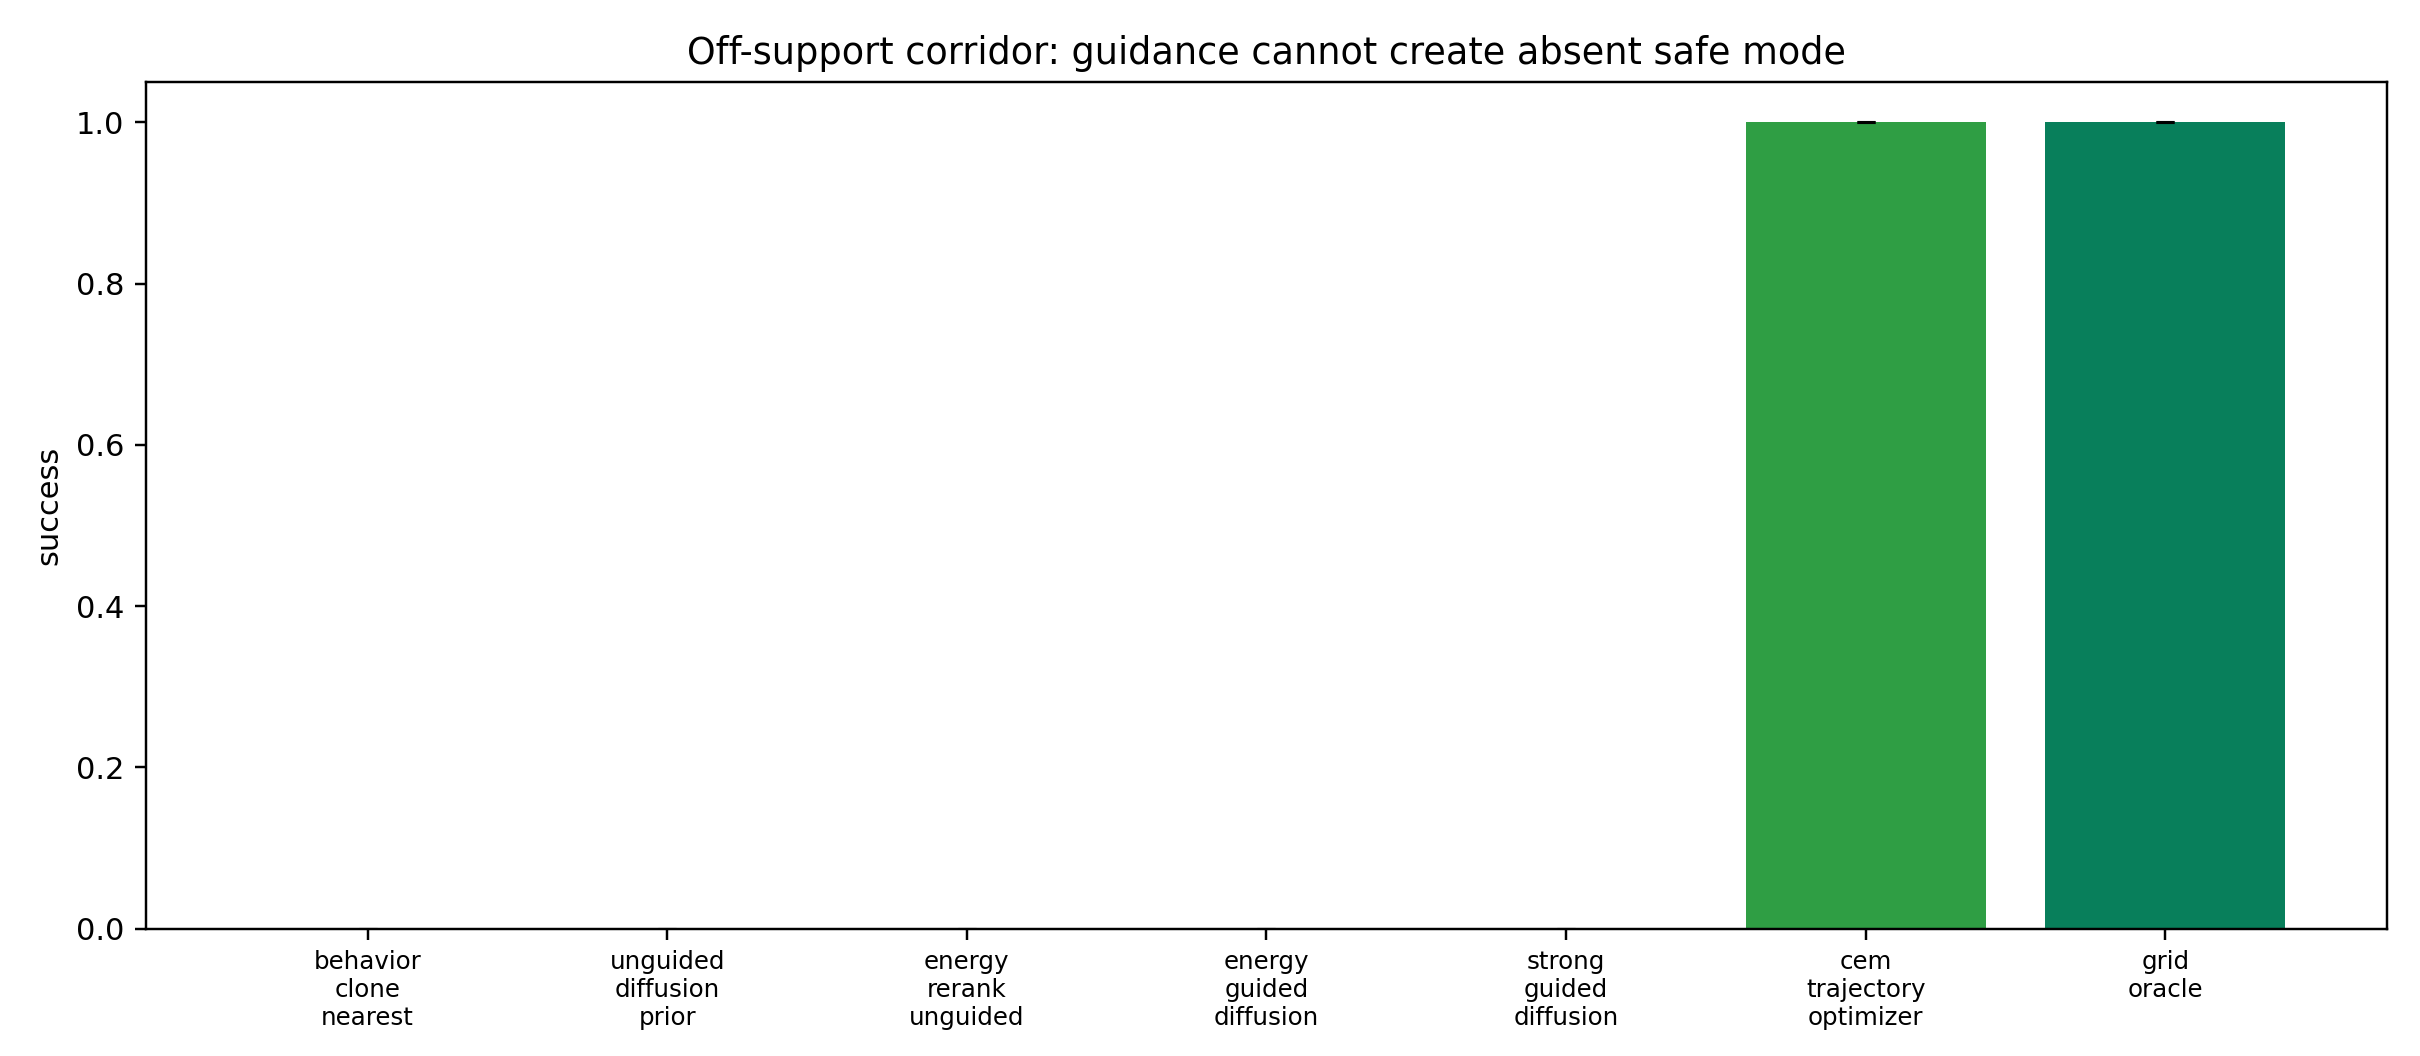
\includegraphics[width=0.95\linewidth]{../figures/diffusion_limit_success.png}
\caption{Off-support success. Energy guidance matches reranking and loses to CEM and the oracle.}
\end{figure}

\begin{figure}[h]
\centering
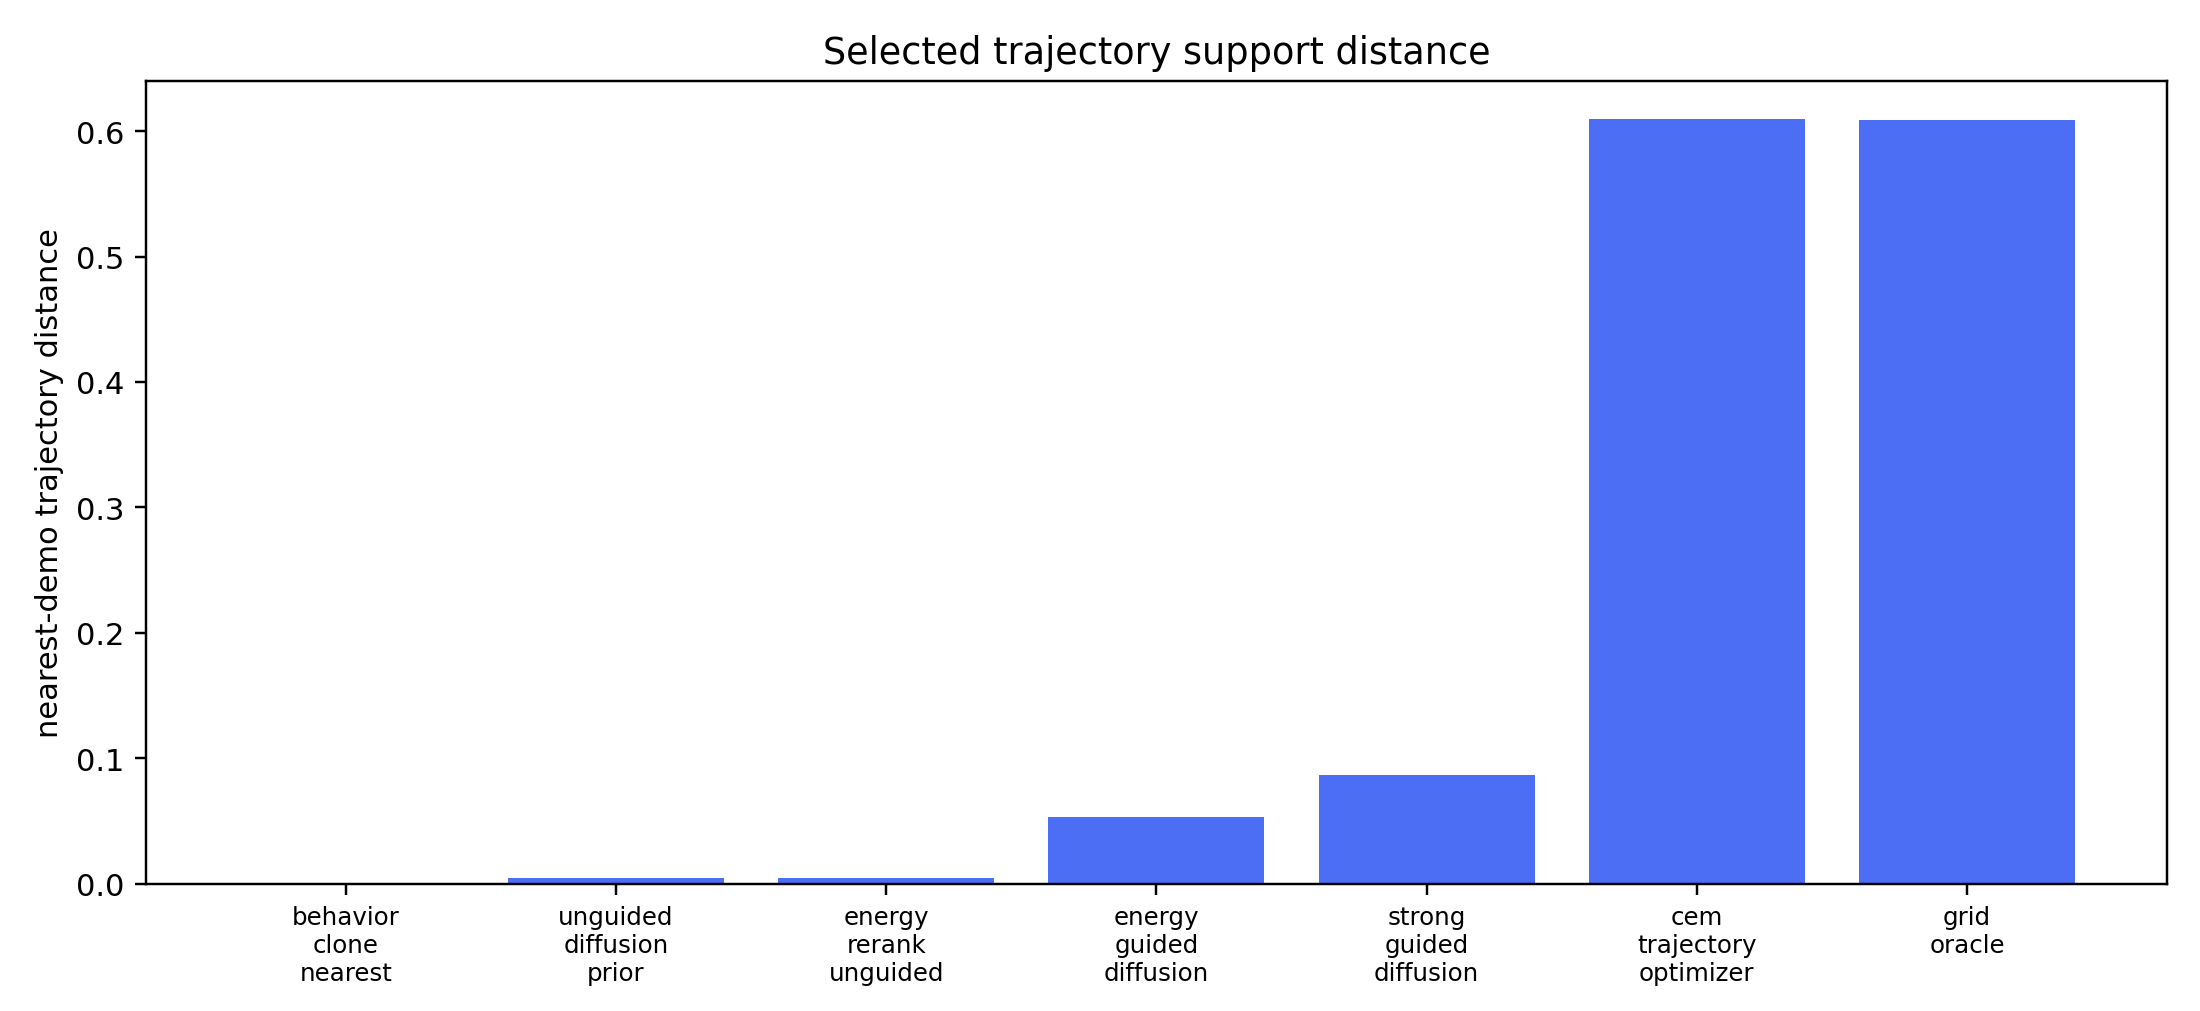
\includegraphics[width=0.95\linewidth]{../figures/diffusion_limit_support_distance.png}
\caption{Support distance of selected trajectories. CEM and oracle leave the demonstration support to find the safe homotopy; guided diffusion remains near the blocked prior.}
\end{figure}

\section{Ablations}
The off-support ablations show why the result is terminal. The full guided method, no-gradient prior sampler, reranking, no-projection guidance, and overguidance all achieve 0.000 success. Strong projection reduces collision but still has 0.000 success and 0.000 mode escape. Removing the prior score produces 0.607 mode escape, but it still has 0.000 success and 0.929 collision. This means unconstrained gradients can leave the prior, but not safely enough to solve the robotics task.

\begin{figure}[h]
\centering
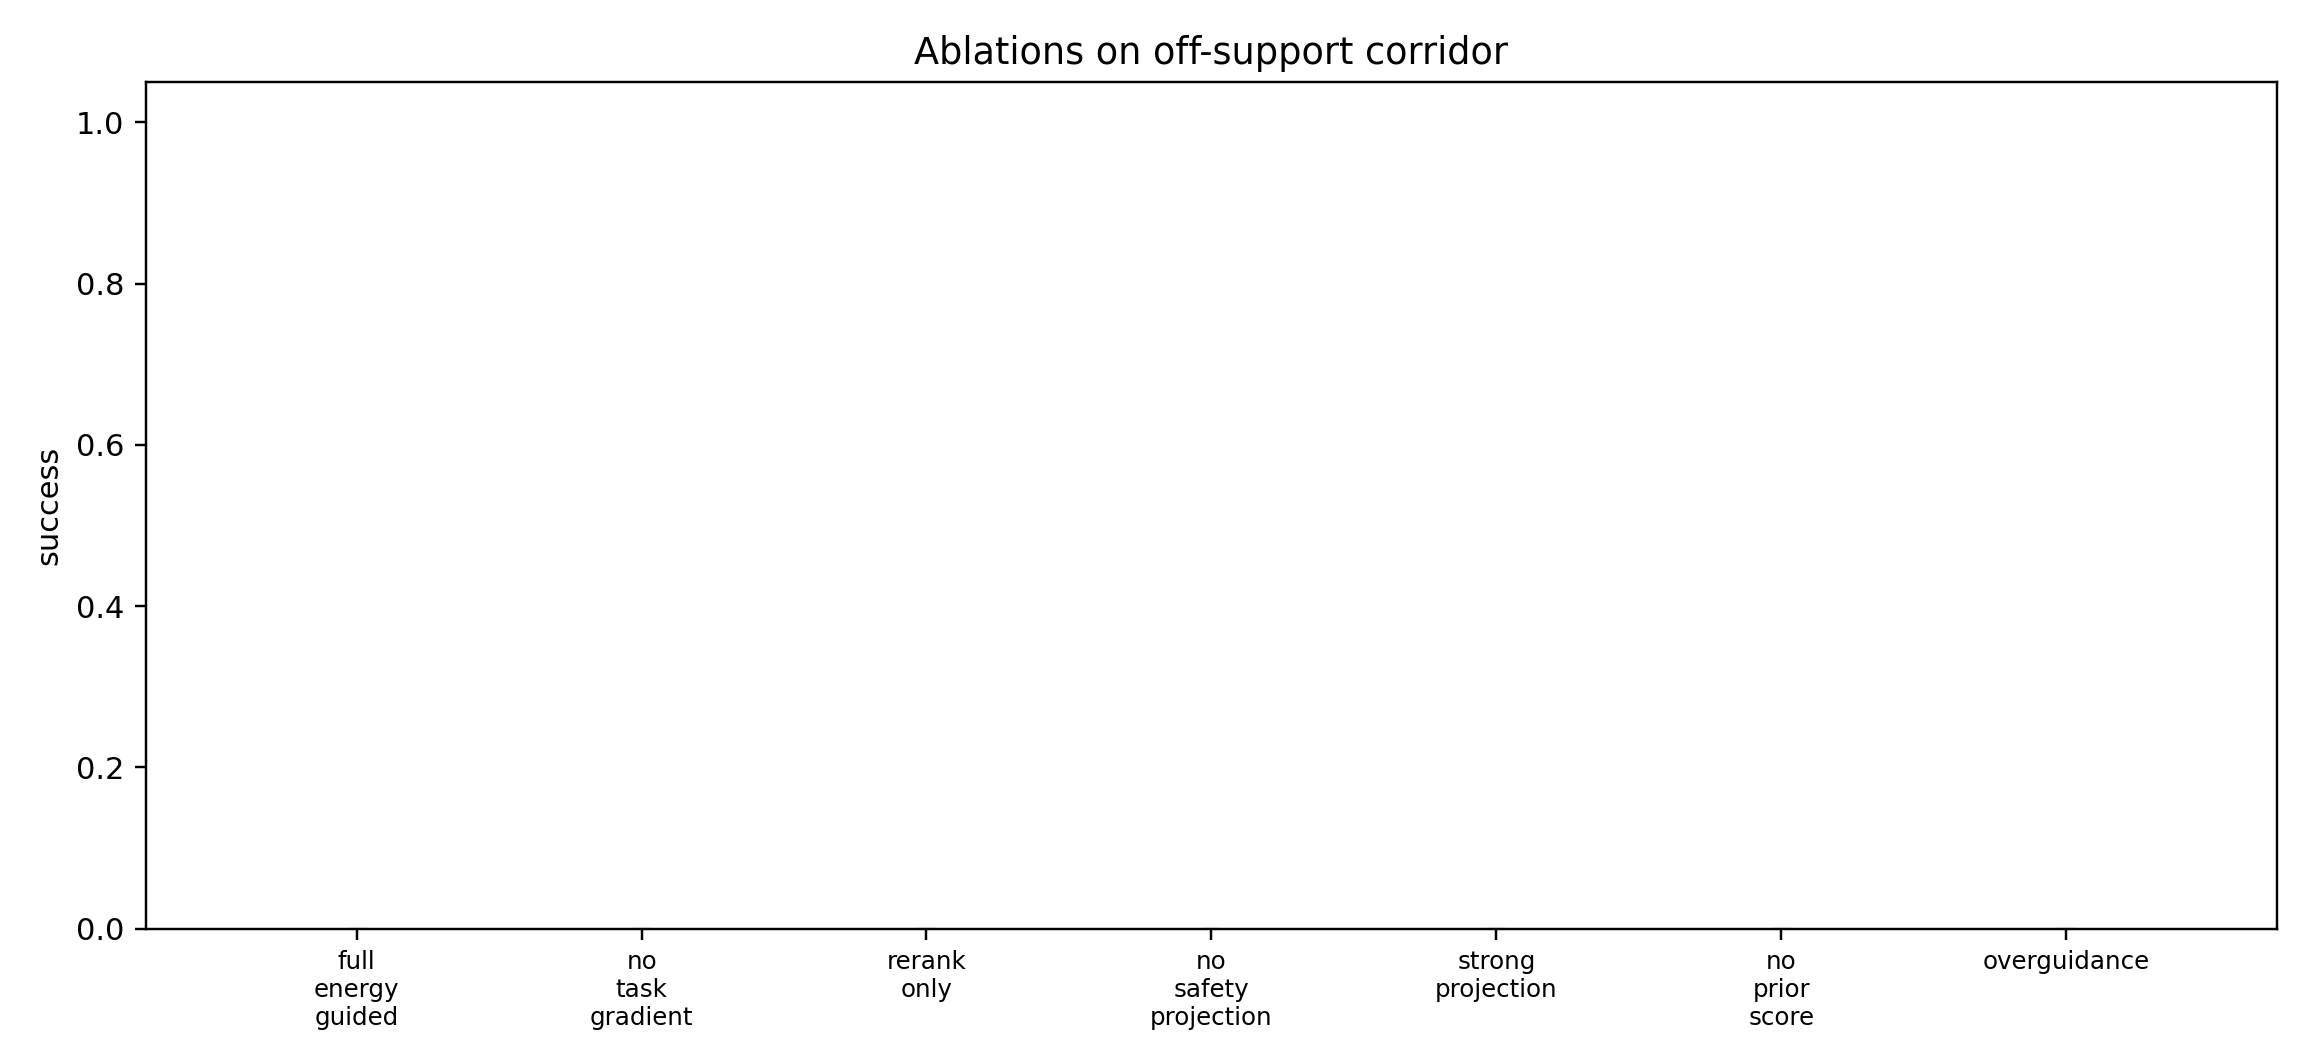
\includegraphics[width=0.95\linewidth]{../figures/diffusion_limit_ablation.png}
\caption{Off-support ablations. The prior traps the sampler; removing the prior causes unsafe escape rather than success.}
\end{figure}

\section{Stress Sweep}
The stress sweep varies the target homotopy frequency from common to absent. At stress level 1.0, the target mode is absent from the prior. \texttt{energy\_rerank\_unguided}, \texttt{energy\_guided\_diffusion}, and \texttt{strong\_guided\_diffusion} all have 0.000 success; CEM and oracle both have 1.000 success.

\begin{figure}[h]
\centering
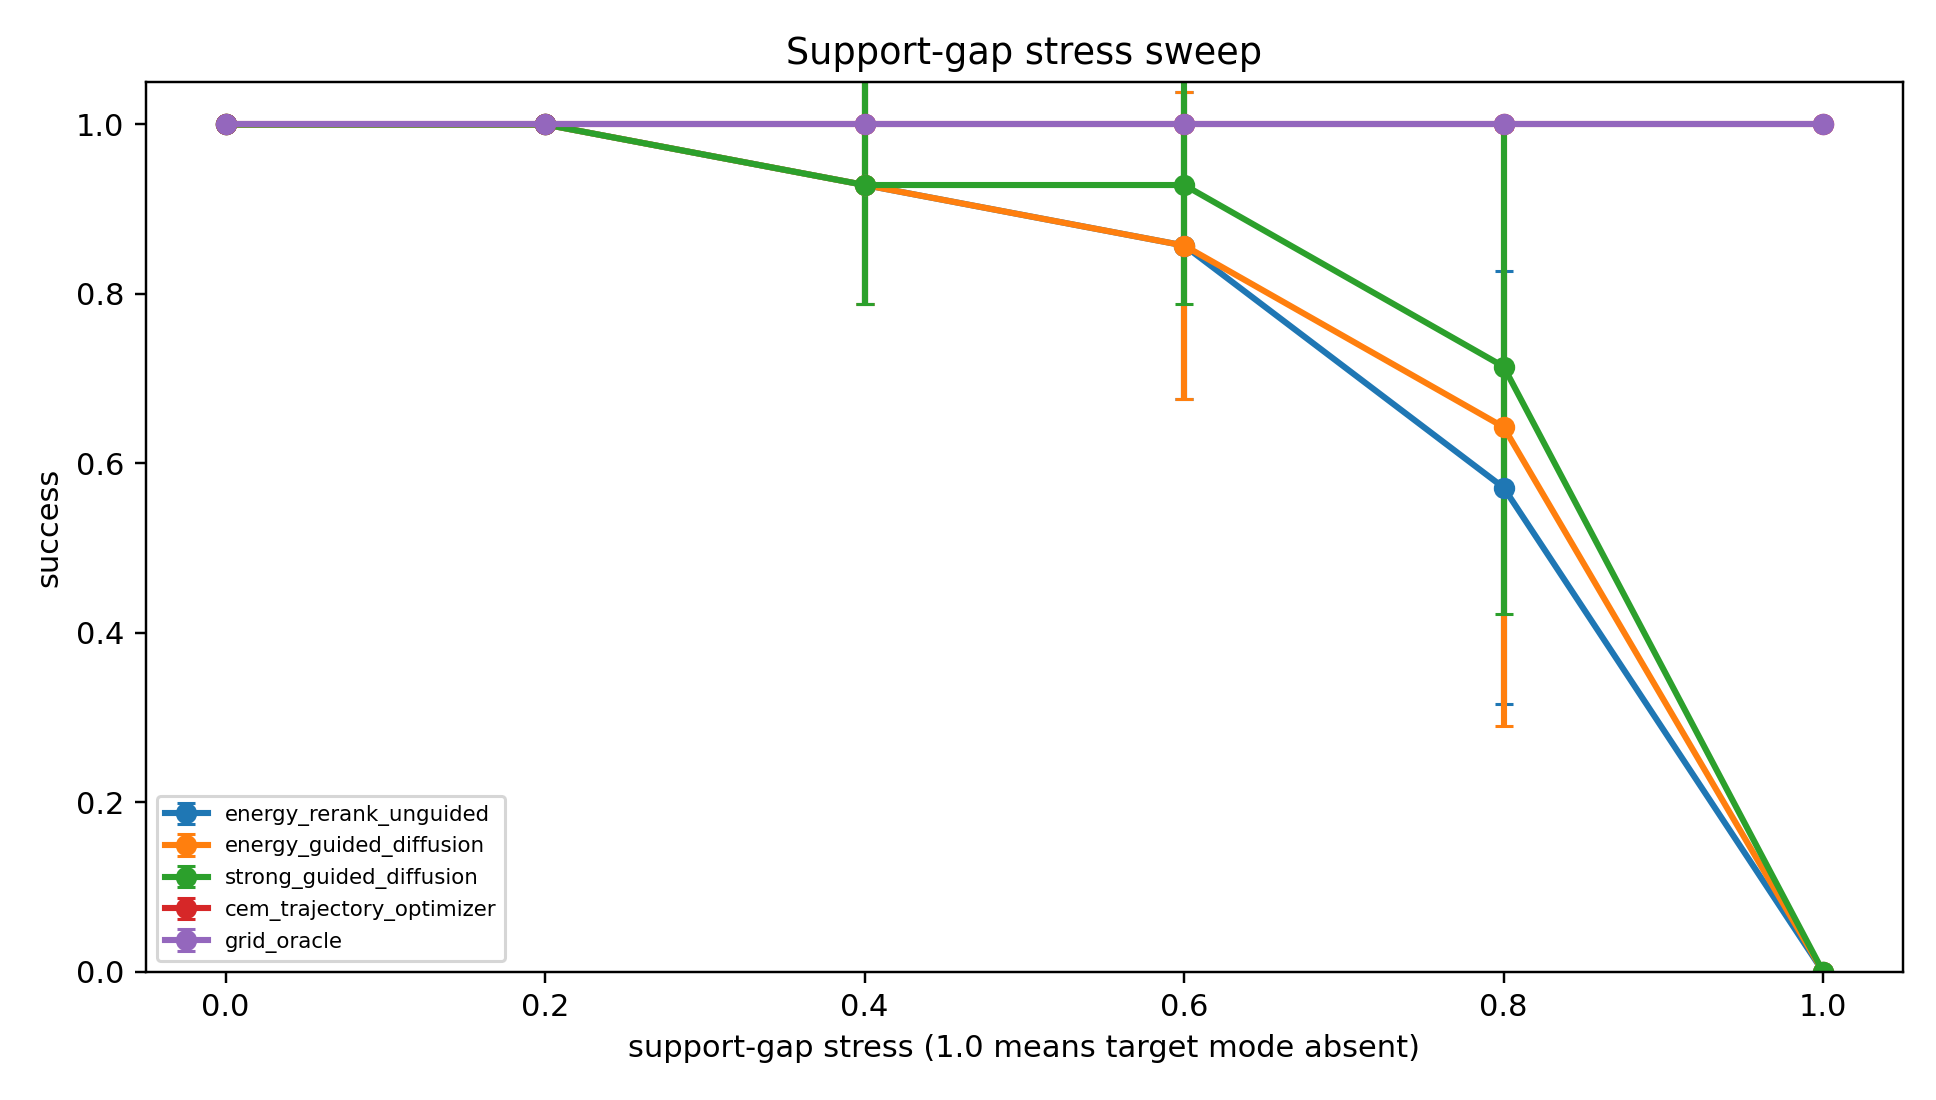
\includegraphics[width=0.95\linewidth]{../figures/diffusion_limit_stress_sweep.png}
\caption{Support-gap stress sweep. Energy-guided diffusion collapses when the required homotopy disappears from the prior.}
\end{figure}

\section{Related Work Pressure}
Energy-guided diffusion and guided robot policies are active areas \citep{prior2,prior4,prior5,prior6}. This makes the novelty boundary demanding: a new paper must show that guidance changes physically reachable behavior, not only that it reweights samples. The local evidence here argues against that stronger claim. Trajectory-optimization baselines also matter because they can construct new homotopies without relying on demonstration support.

\section{Limitations}
This is a local diagnostic benchmark, not a real-robot or high-fidelity simulator study. The diffusion model is a kernel denoising sampler rather than a large neural policy checkpoint. These limitations would prevent an ICLR-main-ready claim even if the method had won. Because the method loses the local benchmark, the archive decision is stronger.

\section{Conclusion}
Paper 78 should not be submitted to ICLR main. The v4 rebuild provides implemented evidence, but the evidence is negative: energy guidance does not safely create missing diffusion-policy support and does not beat reranking or CEM. The correct terminal state is \textbf{KILL/ARCHIVE}.

\bibliographystyle{iclr2026_conference}
\bibliography{references}

\end{document}
